\chapter{Data Results}
After closure of the background estimation procedure within control regions, 
we first apply the background estimate to a loose selection that contains all of the full selection cuts with the exception of subjet 
b-tagging and N-subjettiness.  The agreement using this selection can be seen in figure \ref{figs:CMSTTonlyMtbvsBkg1}.

\begin{figure}[htcb]
\begin{center}
\subfigure{\label{figs:CMSTTonlyMtbvsBkg_BifPoly_fit}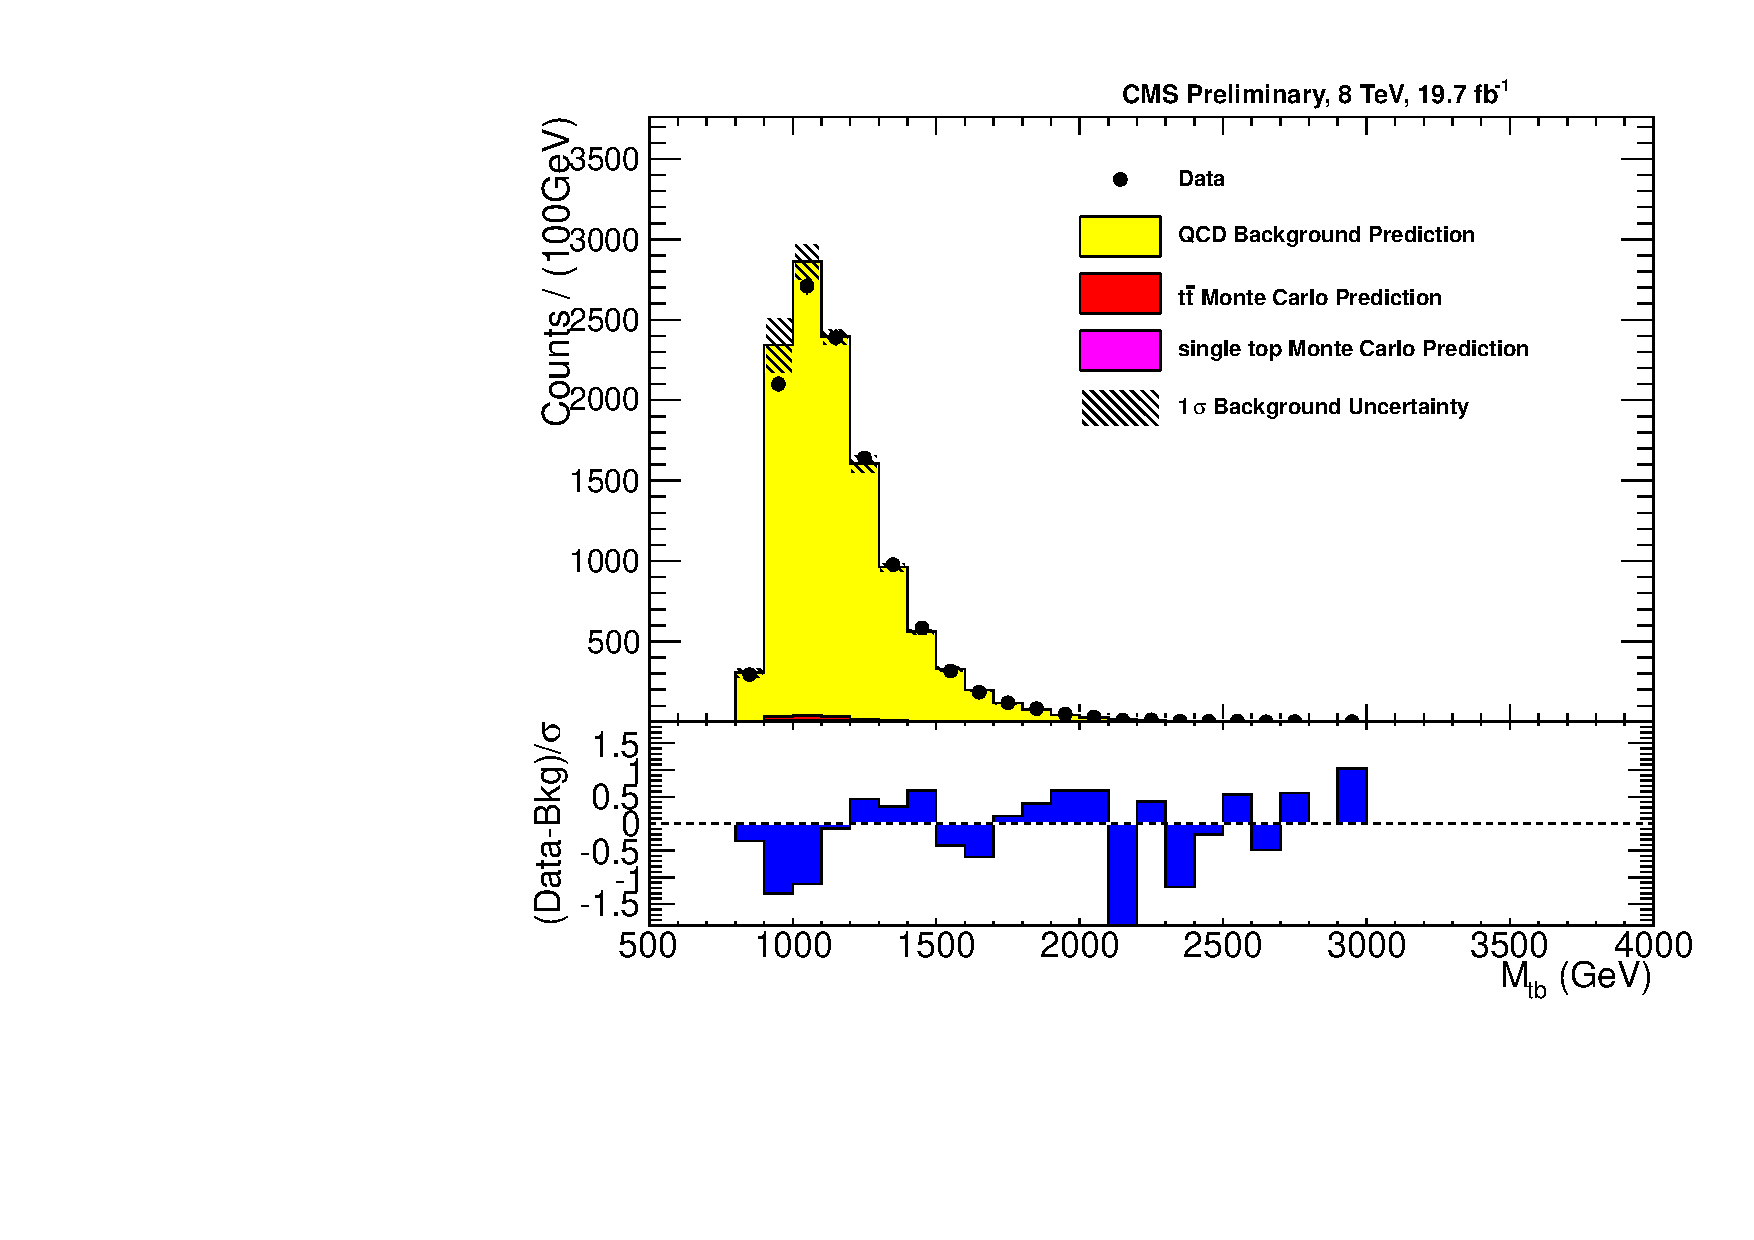
\includegraphics[width=0.7\textwidth]{AN-13-004/figs/CMSTTonlyMtbvsBkg_BifPoly_fit.pdf}}\\
\subfigure{\label{figs:CMSTTonlyMtbvsBkgsemilog_BifPoly_fit}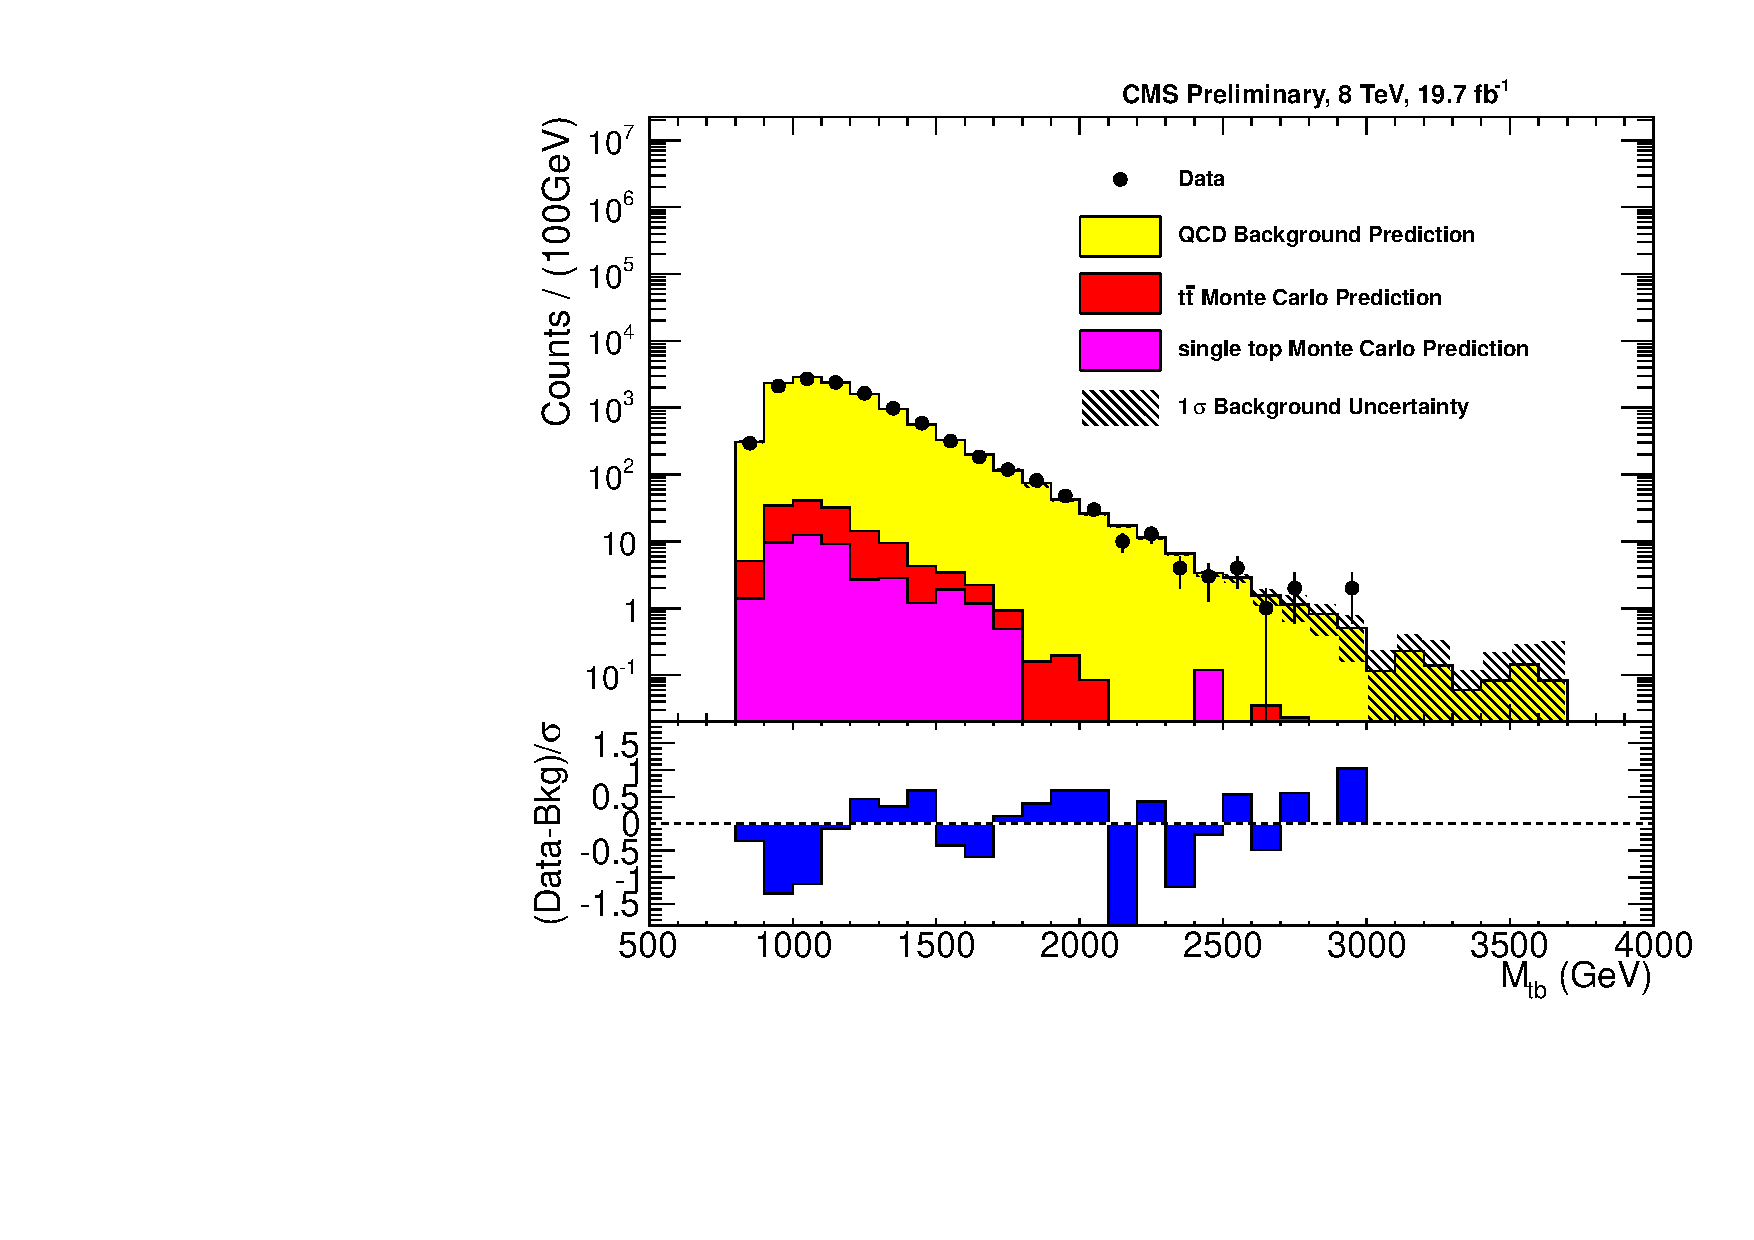
\includegraphics[width=0.7\textwidth]{AN-13-004/figs/CMSTTonlyMtbvsBkgsemilog_BifPoly_fit.pdf}}
\caption{
A plot of the full selection before N-subjettiness and subjet b-tagging discrimination.   
Here we investigate the data-background agreement in a loose selection before looking at the full top tagging selection.  Top and bottom plots are the same but with linear and log y-axis scale.}
\label{figs:CMSTTonlyMtbvsBkg1}
\end{center}
\end{figure}

After observing agreement is the loose selection, we investigate the full selection.  The final results are shown in Figure \ref{figs:MtbvsBkg1}.  We proceed to compute 
limits on the $\wpr$ cross-section.  Background estimation of selected relevant variables can be seen in 
Figures \ref{figs:kinplotsdata1} and \ref{figs:kinplotsdata2}.

\begin{figure}[htcb]
\begin{center}
\subfigure{\label{figs:MtbvsBkg_BifPoly_fit}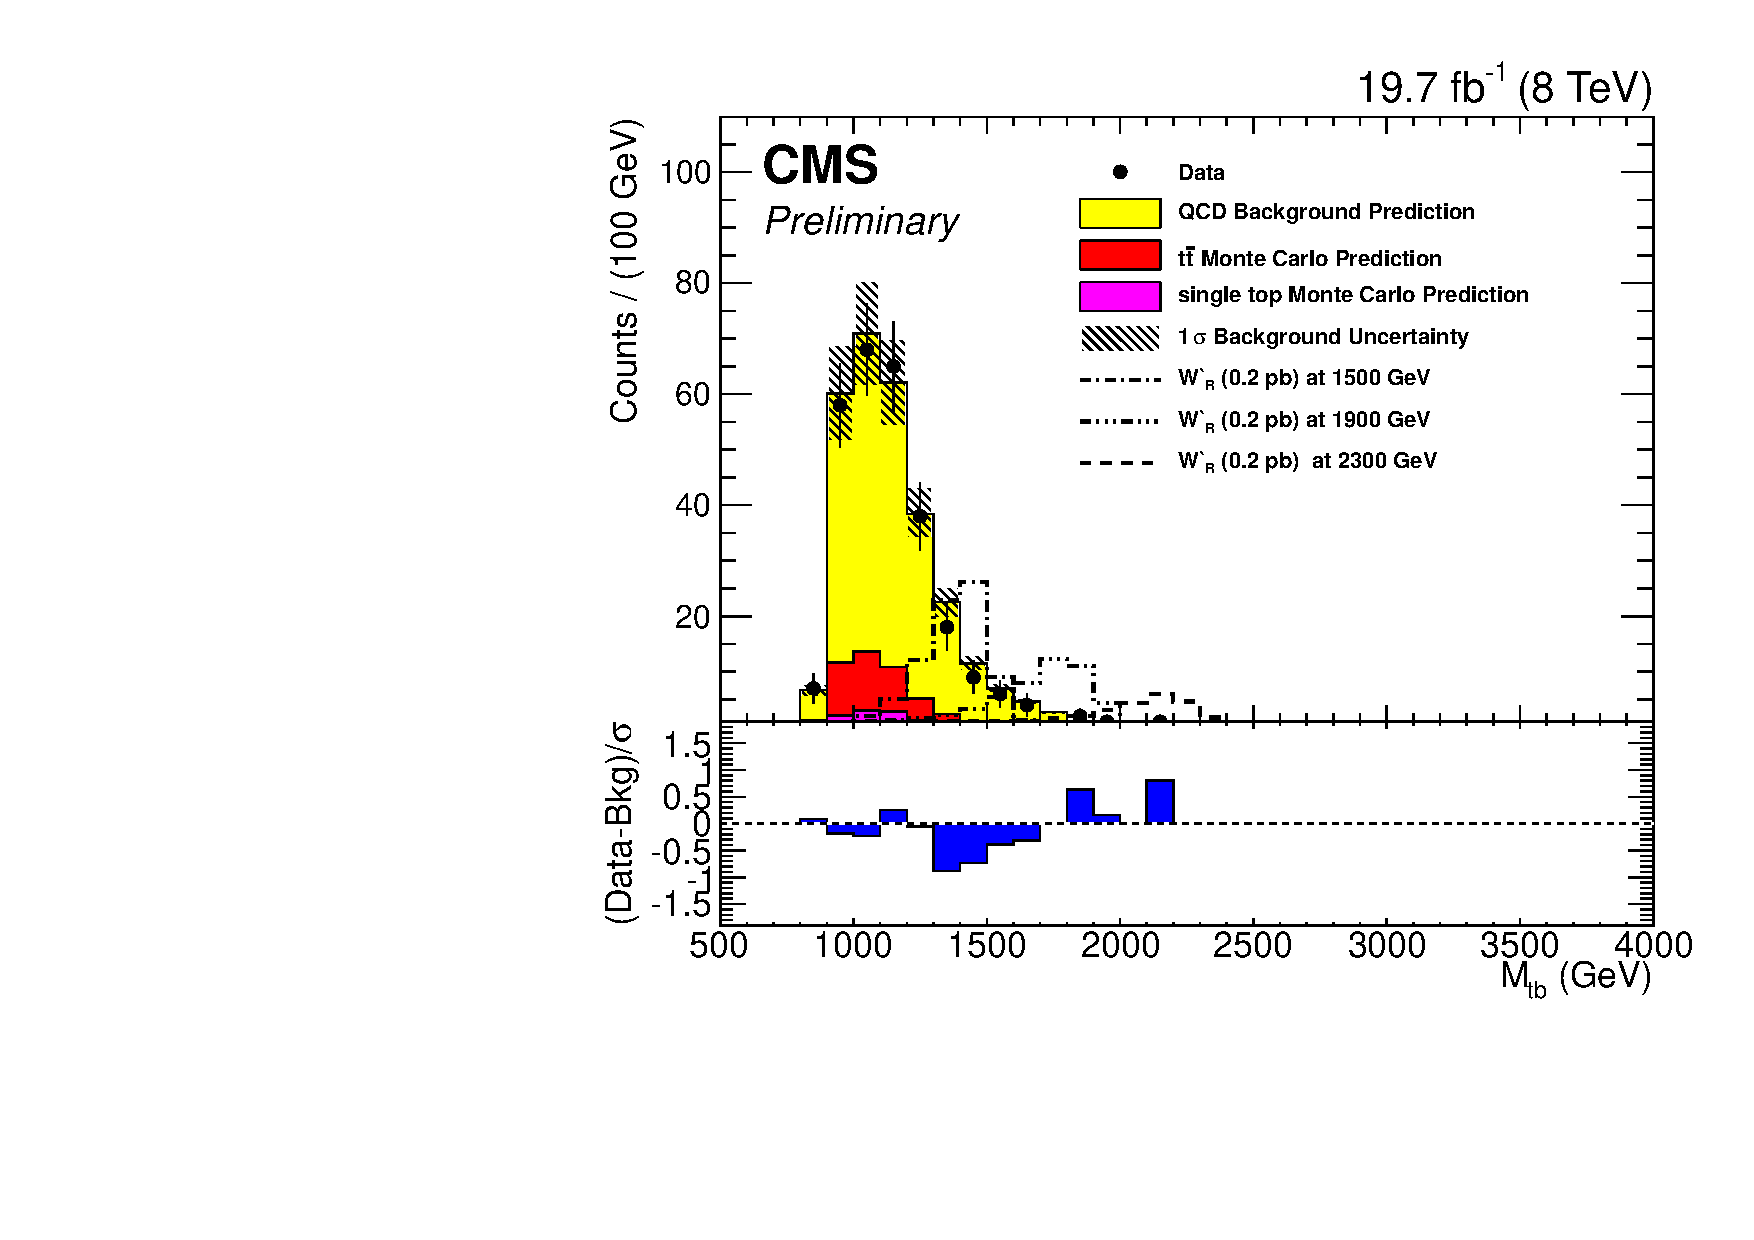
\includegraphics[width=0.7\textwidth]{AN-13-004/figs/MtbvsBkg_BifPoly_fit.pdf}}\\
\subfigure{\label{figs:MtbvsBkgsemilog_BifPoly_fit}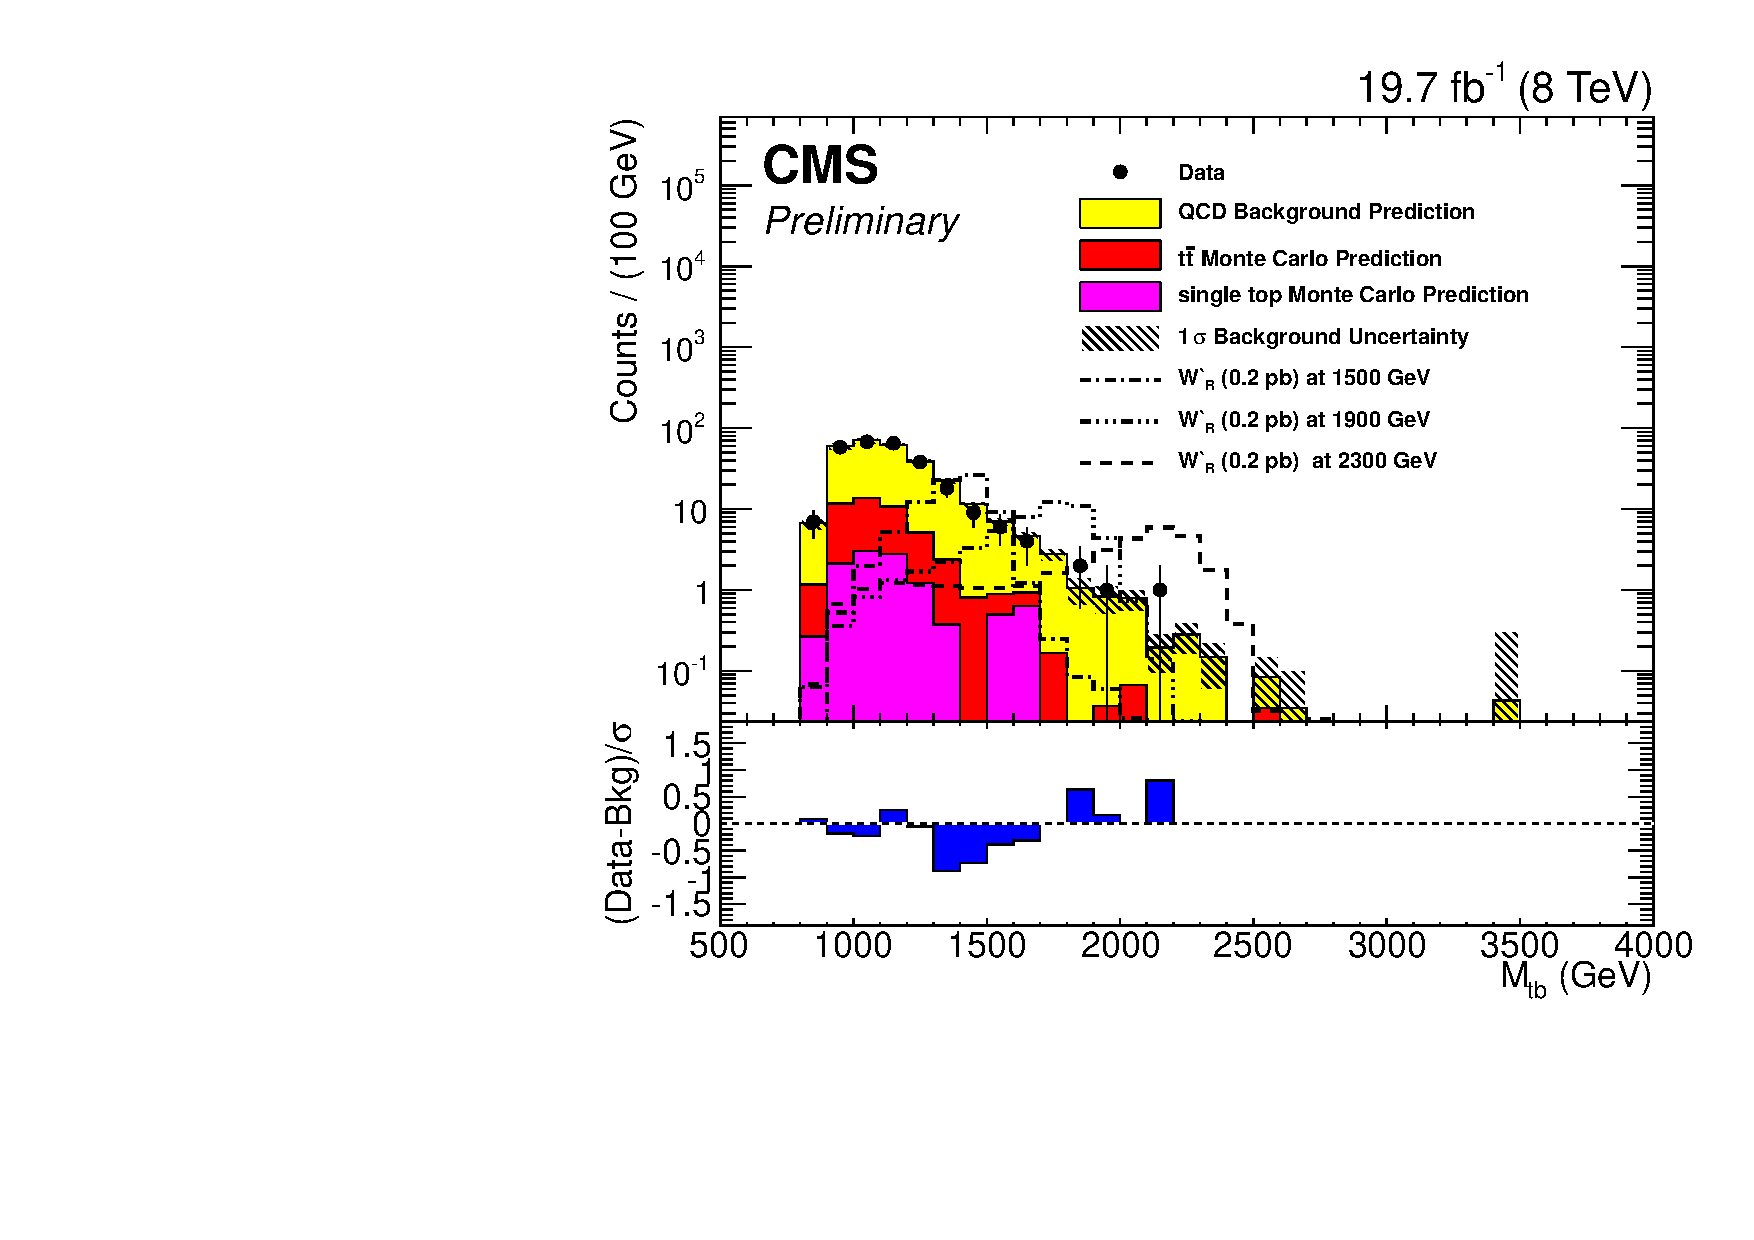
\includegraphics[width=0.7\textwidth]{AN-13-004/figs/MtbvsBkgsemilog_BifPoly_fit.pdf}}
\caption{
A plot of the full selection comparing data, signal and background.  
The single top contribution is not considered when setting limits.  
The normalization for the signal samples is set to a cross-section of 0.2 pb.  Top and bottom plots are the same but on linear and log y-axis scale.}
\label{figs:MtbvsBkg1}
\end{center}
\end{figure}

\begin{figure}[htcb]
\centering
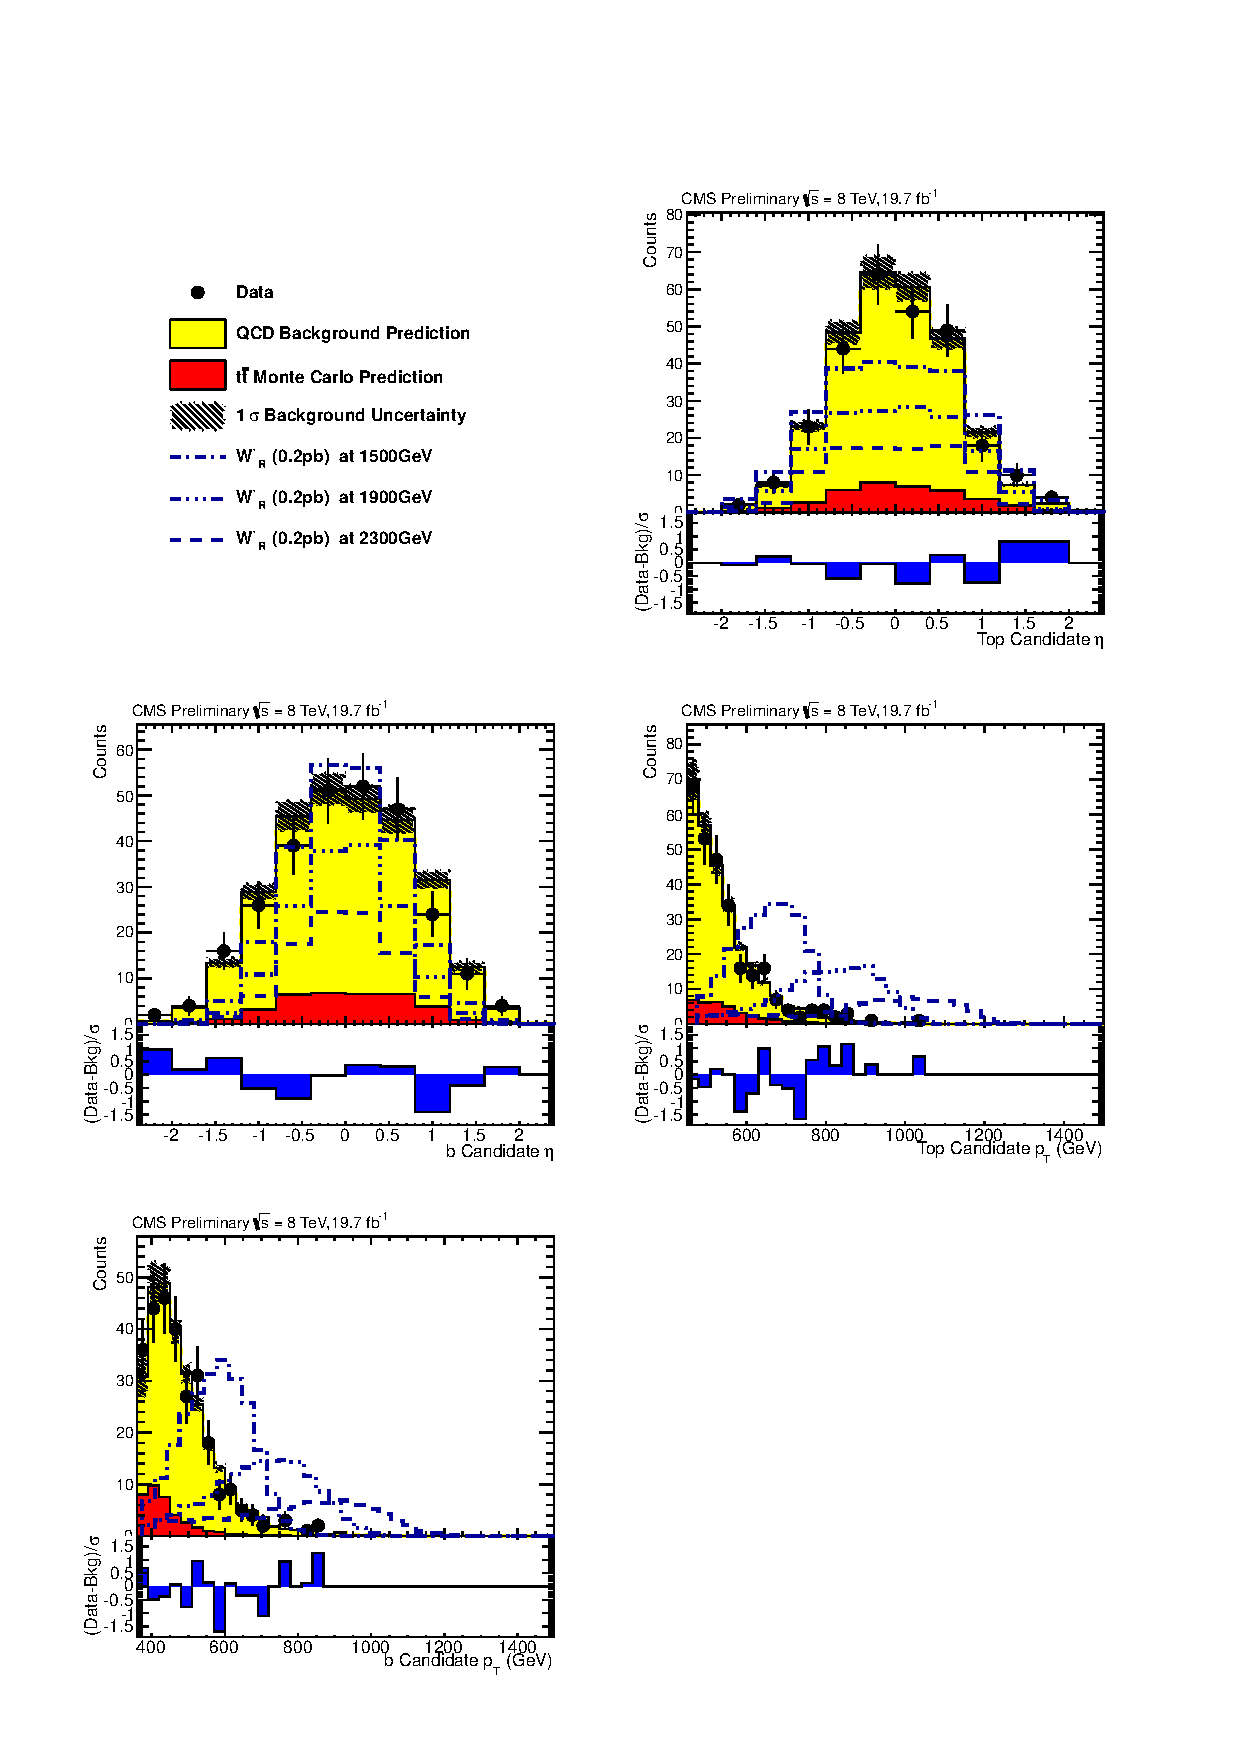
\includegraphics[width=.7\textwidth]{AN-13-004/figs/KinPlots_Data1.pdf}
\caption{Background estimation of kinematic variables.  The error bars shown are from the three primary sources; uncertainty on the fit, choice of fit, $\ttbar$ normalization, and $\ttbar$ $Q^2$ uncertainty}
\label{figs:kinplotsdata1}
\end{figure}  
\clearpage

\begin{figure}[htcb]
\centering
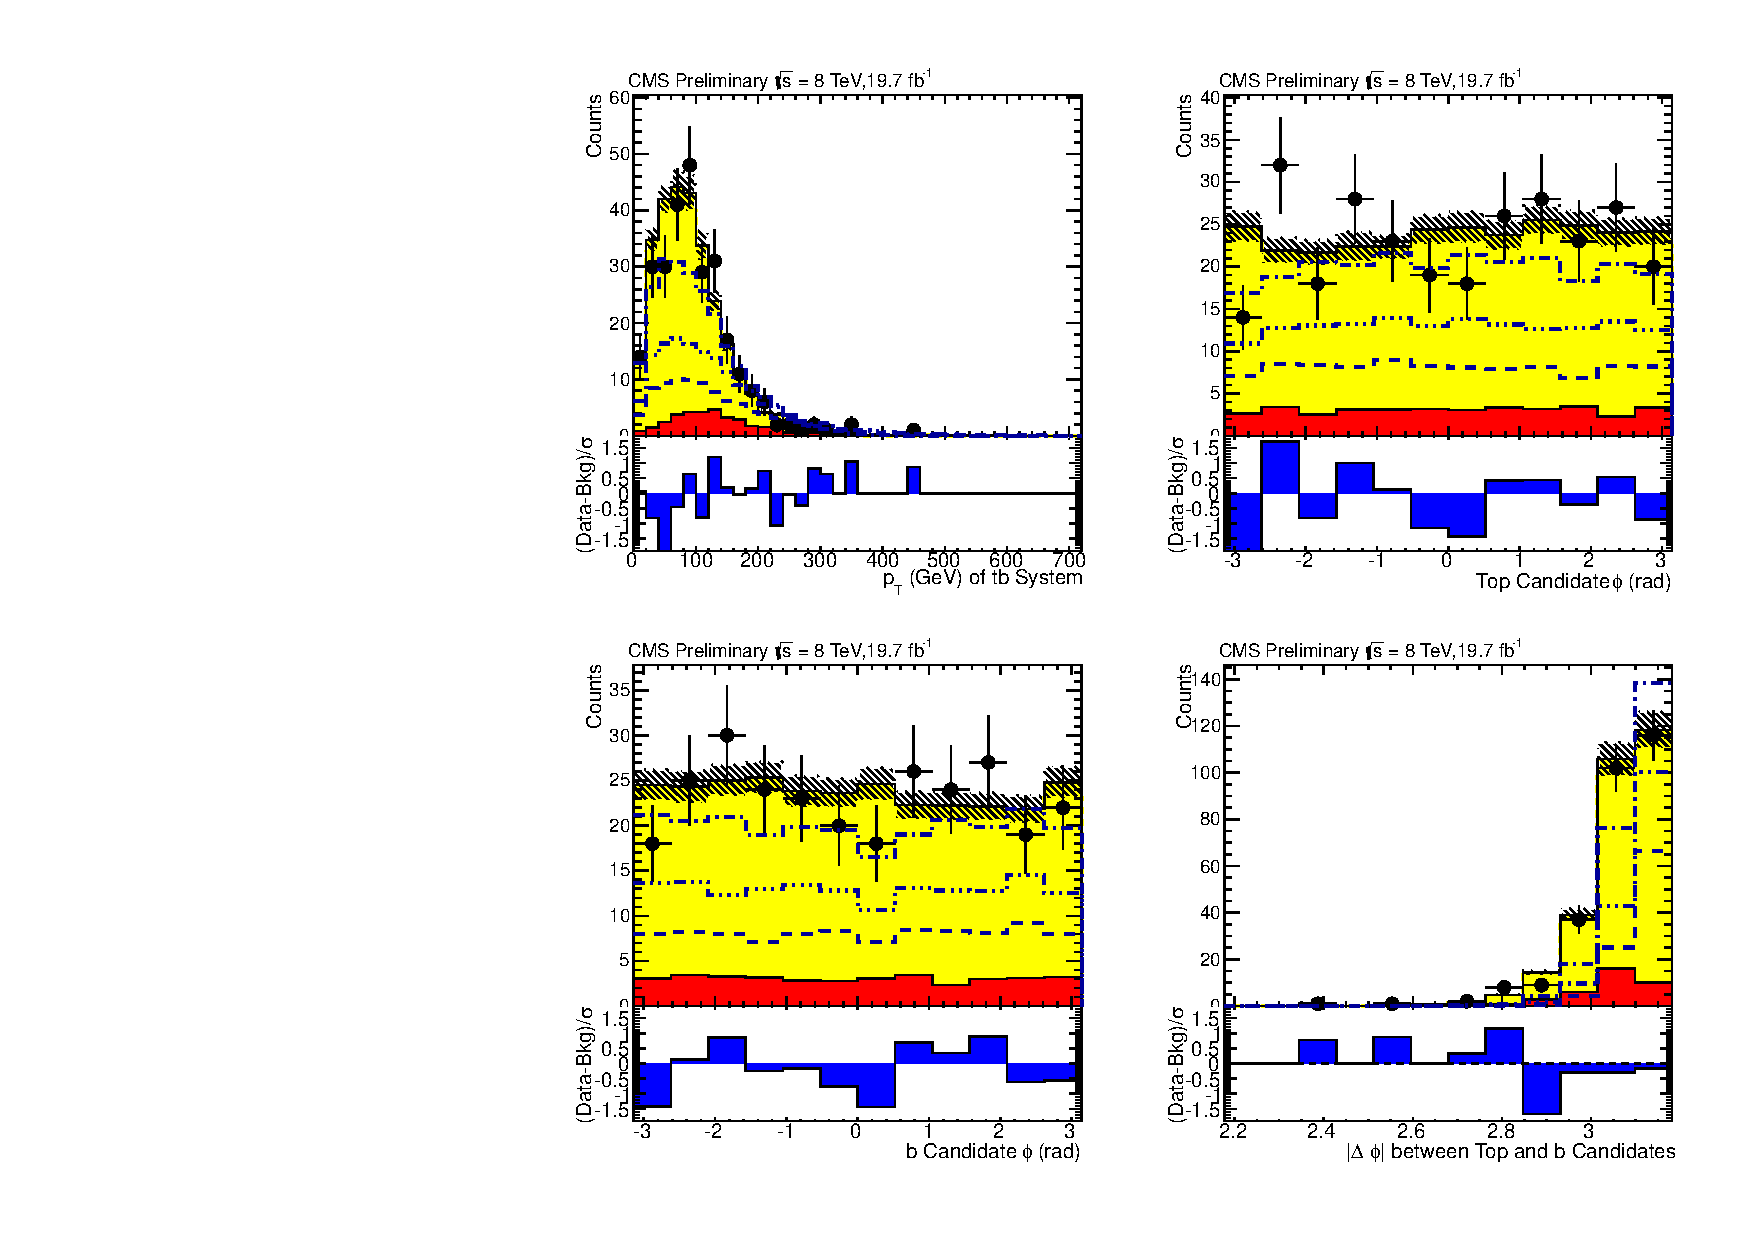
\includegraphics[width=.7\textwidth]{AN-13-004/figs/KinPlots_Data2.pdf}
\caption{Background estimation of kinematic variables.  The error bars shown are from the three primary sources; uncertainty on the fit, choice of fit, $\ttbar$ normalization, and $\ttbar$ $Q^2$ uncertainty}
\label{figs:kinplotsdata2}
\end{figure}  
\clearpage

